\documentclass{article}

\usepackage[pdfauthor={CoderDojo Linz},
            pdftitle={halloween-puzzle}]
            {hyperref}

\newcommand{\footertitle}{Halloween Puzzle}
% settings.tex
\usepackage[
    a4paper, 
    top=2cm,
    left=1cm,
    right=1cm,
    bottom=2cm
]{geometry}

\usepackage{fontspec}
\usepackage{graphicx}
\usepackage{hyperref}
\usepackage{fancyhdr}
\usepackage[ngerman]{babel}
\usepackage{wrapfig}
\usepackage{enumitem}
\usepackage{titlesec} 
\usepackage{ragged2e}
\usepackage{tcolorbox}
\usepackage{array}
\usepackage[table]{xcolor}
\usepackage{fontawesome5}

\setmainfont{Carlito}

% Fancyhdr setup
\fancypagestyle{defaultpagestyle}{
    \fancyhf{} % Clear all headers and footers
    \fancyhead[C]{
\includegraphics[width=5cm]{../../CoderDojo_Logo.png}} 
    \renewcommand{\headrulewidth}{0pt} % Remove header line
    \renewcommand{\footrulewidth}{0pt} % Remove footer line
    \fancyfoot[L]{\footertitle}
    \fancyfoot[R]{Seite \thepage} % Right footer with page number
}

\newcommand{\SectionDesign}[4]{
    \noindent
    \csname #1*\endcsname{\textcolor[HTML]{1E90FF}{\fontsize{#2pt}{#3pt}\selectfont #4}}
}

\newcommand{\TextAndImage}[5][{}]{
    \fontsize{11pt}{16pt}\selectfont
    \noindent
    \begin{minipage}[c]{#4\textwidth}
    \RaggedRight
    #2 % First parameter: text
    \end{minipage}
    \hfill
    \begin{minipage}[c]{#5\textwidth}
    \includegraphics[width=\textwidth, #1]{#3} % Second parameter: image file name
    \end{minipage}
}

\newcommand{\ImageAndText}[2]{
    \fontsize{16pt}{24pt}\selectfont
    \noindent
    \begin{minipage}[c]{0.65\textwidth}
        \includegraphics[width=\textwidth]{#1} % Second parameter: image file name
    \end{minipage}
    \hfill % Fills the space between the minipages
    \begin{minipage}[c]{0.25\textwidth}
        \centering
        #2 % First parameter: text
    \end{minipage}
}

\newcommand{\TextDesign}[1]{
    \fontsize{11pt}{16pt}\selectfont
    \noindent
    \RaggedRight
    #1 % First parameter: text
}
\graphicspath{{images/}}

\begin{document}
    \pagestyle{defaultpagestyle}

    \SectionDesign{section}{24}{24}{\textbf{Halloween Puzzle}}

    \SectionDesign{subsection}{18}{24}{\textbf{Einleitung}}
    
    \TextDesign{
    Willkommen beim Halloween Puzzle! Diese Übung eignet sich gut für alle, die zwar schon einiges mit Scratch gemacht, jedoch noch wenig oder keine Erfahrung mit textueller Programmierung haben. Wir wollten gemeinsam ein \textit{Halloween Puzzle} bauen, bei dem man Punkte sammeln kann, indem man mindestens drei gleiche Symbole zusammenbringt. Als Programmiersprache werden wir \textit{TypeScript} verwenden.
    }

    \SectionDesign{subsection}{18}{24}{\textbf{Entwicklungsumgebung laden}}
    
    \TextDesign{
    Als erstes müssen wir die \textit{Entwicklungsumgebung} laden. Dafür brauchst du eine moderne Version von dem Internetbrowser \textit{Chrome} oder \textit{Edge}. Starte den Browser und öffne die folgende Webseite:
    }

    \href{https://stackblitz.com/edit/digiferien-2024-starter}{\textcolor{blue}{https://stackblitz.com/edit/digiferien-2024-starter}}

    \vspace{0.5cm}
    \TextDesign{
    Wenn alles klappt, dann solltest du unsere Entwicklungsumgebung \textit{Stackblitz} sehen. Sie sieht in etwa so aus:
    }

    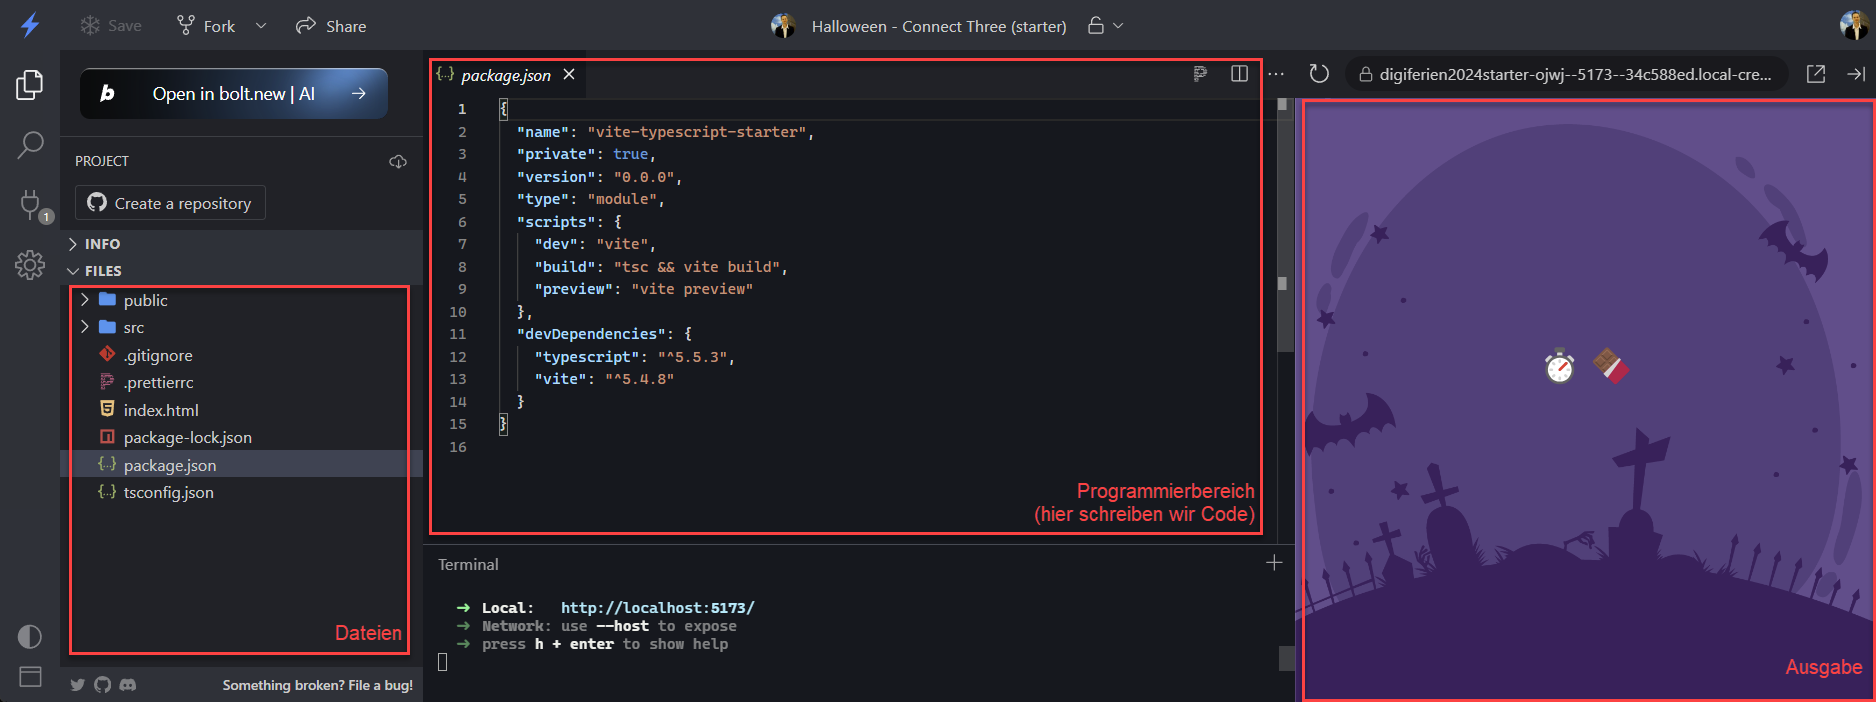
\includegraphics[width=\textwidth]{stackblitz.png}
    \vspace{0.5cm}
    
    \TextAndImage{
    Du musst einmal auf \textit{Fork} klicken, damit du deine eigene Kopie von dem Spiel bekommst. \textbf{Lade zur Sicherheit danach den Inhalt des Internetbrowsers einmal neu.}
    }{fork.png}{0.55}{0.40}{11}{16}

    \newpage

    \SectionDesign{subsection}{18}{24}{\textbf{Hintergrund ändern}}
    
    \TextDesign{
    Fangen wir mit ersten, einfachen Programmierschritten an. Deine Aufgabe ist es, den Hintergrund für unser Spiel zu wählen. Öffne dafür die Datei \textit{style.css} im Ordner \textit{src}, indem du sie anklickst. Ganz oben findest du einen Hinweis, was du ändern musst, um verschiedene Hintergründe auszuwählen. Die folgende Grafik zeigt auch, wo du etwas ändern musst. Probiere die Hintergründe \textit{bg1.png} bis \textit{bg6.png} aus. Wähle den Hintergrund, der dir am besten gefällt.
    }
    
    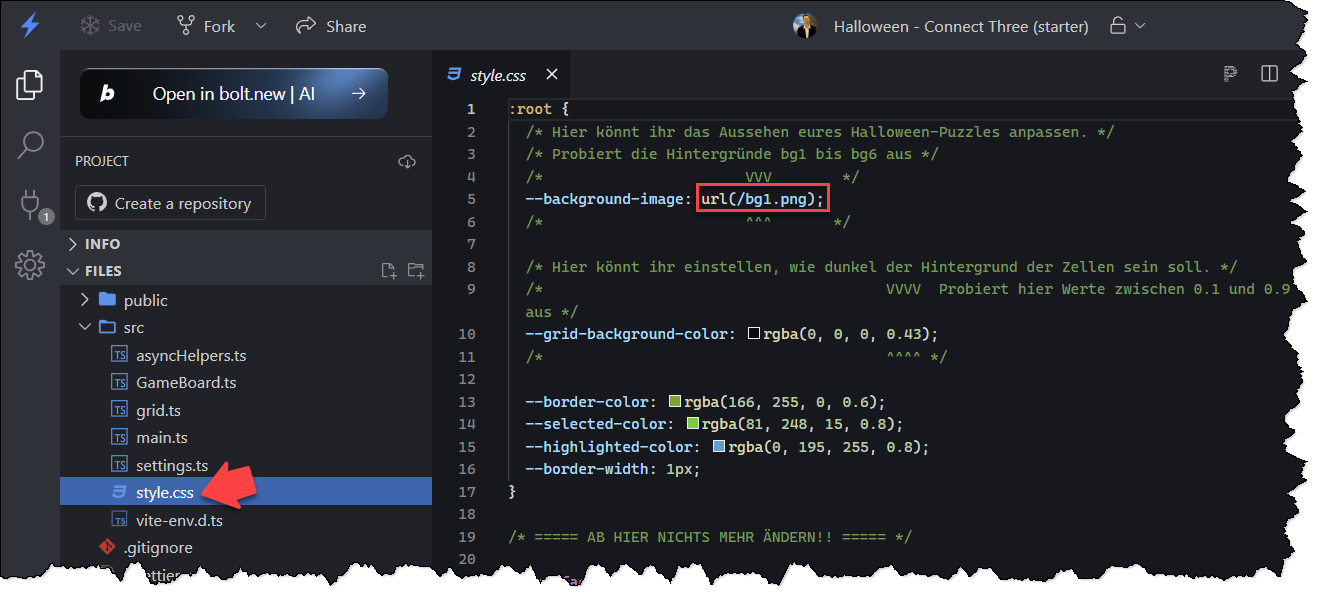
\includegraphics[width=\textwidth]{background.png}
        
    \TextDesign{
    Wenn du genau schaust, dann siehst du, dass in der \textit{style.css}-Datei noch weitere Einstellungen, die du ändern kannst. Lass sie im Moment noch so wie sie sind. Wir kommen später auf sie zurück.
    }

    \TextDesign{
    \textbf{Tipp: }Wenn du etwas im Code änderst, aktualisiert sich die Ausgabe automatisch. Dafür ist kein explizites Speichern notwendig. \textbf{Trotzdem ist es empfehlenswert, öfter auf \textit{Save} zu klicken.} Wenn nämlich dein Programm abstürzt und du den Browser neu landen musst, wird der Code auf den letzten Stand zurückgesetzt, den du gespeichert hast.
    }

    \TextAndImage{
    \textbf{Tipp: }Wenn du etwas im Code änderst, aktualisiert sich die Ausgabe automatisch. Dafür ist kein explizites Speichern notwendig. Falls das automatische Aktualisieren einmal nicht klappt, blende die Ausgabe einmal aus- und dann wieder ein (siehe Bild rechts). Spätestens dann solltest du die neue Ausgabe sehen.
    }{output-show-hide.png}{0.55}{0.40}{11}{16}

    \vspace{0.5cm}
    \ImageAndText{save.png}{
    \textbf{Trotzdem ist es empfehlenswert, öfter auf \textit{Save} zu klicken} (siehe Bild links). Wenn nämlich dein Programm abstürzt und du den Browser neu landen musst, wird der Code auf den letzten Stand zurückgesetzt, den du gespeichert hast.
    }{0.40}{0.55}{11}{16}

    \newpage

    \SectionDesign{subsection}{18}{24}{\textbf{Raster anzeigen}}

    \TextAndImage{
    Jetzt legen wir mit TypeScript los. Ein Spiel wie das Halloween Puzzle von Grund auf zu programmieren ist nicht einfach. Das würde zu lange dauern. Daher haben wir einiges für dich vorbereitet. Du musst den Code in der Datei \textit{main.ts} vervollständigen. Diese Anleitung führt dich durch alle notwendigen Schritte.

    \vspace{0.5cm}

    Öffne die Datei \textit{main.ts} über das Dateifenster (siehe Bild rechts). Falls du einen relativ kleinen Bildschirm hast, kannst du anschließend das Dateifenster ausblenden, da wir uns im Moment ganz auf \textit{main.ts} konzentrieren.
    }{main-open.png}{0.40}{0.55}{11}{16}

    \vspace{0.5cm}
    
    \TextDesign{
    Suche die Funktion \textit{buildGrid()} in deinem Programm. Die Zeile die du suchst, enthält \textit{function buildGrid() \{}. Hier ist der Code, den du \textbf{innerhalb der geschweiften Klammern} von \textit{buildGrid()} eintippen musst.

    \vspace{0.5cm}

    \textbf{Tipp: }Die Zeilen, die mit \textit{//} beginnen, sind \textit{Kommentare}. Man verwendet sie, um sich Notizen zu machen. Du musst die Kommentarzeilen \textbf{nicht} abschreiben. Sie sollen dir nur erklären, was der Code macht. Wenn du etwas nicht verstehst, frag erfahrene Programmiererinnen oder Programmierer im CoderDojo oder in der Schule.
    }

    \begin{lstlisting}[language=JavaScript]
function buildGrid() {
  // Der "for"-Befehl ist eine sogenannte Schleife. Vielleicht kennst du Schleifen 
  // aus Scratch. Dort heißen sie "Wiederhole fortlaufend", "Wiederhole bis", 
  // "Wiederhole ___ mal", etc.

  // Diese Schleife wird je Zeile wiederholt. "SIZE_Y" ist eine sogenannte "Konstante".
  // Sie legt fest, wie viele Zeilen wir haben (in unserem Fall 10).
  for (let row = 0; row < SIZE_Y; row++) {
    // Diese Schleife wird je Spalte wiederholt. "SIZE_X" ist wie oben eine Konstante,
    // die die Anzahl der Spalten festlegt (in unserem Fall 6).
    for (let col = 0; col < SIZE_X; col++) {
      // Diese Funktion fügt eine Zelle zu unserem Raster hinzu. Dabei übergeben
      // wir unter andere die Spalte ("col" Abkürzung für "column") und die Zeile ("row").
      addCell(grid, col, row);
    }
  }
}
    \end{lstlisting}

    \newpage

    \TextDesign{
    Geschafft? Super! Jetzt probieren wir das aus. Suche dir die Funktion \textit{startup()} heraus. Sie ist direkt über der Funktion \textit{buildGrid}, die du gerade geändert hast. Schreib in \textit{startup} die folgenden Befehle:
    }

    \begin{lstlisting}[language=JavaScript]
async function startup() {
  // Der Code in dieser Funktion wird am Beginn des Programms ausgeführt.

  // Als erstes müssen wir das Styling initialisieren. Das ist ein technisches Detail,
  // auf das wir hier nicht näher eingehen werden.
  initializeStyling();

  // Jetzt erstellen wir das Raster
  buildGrid();
}
    \end{lstlisting}

    \TextAndImage{
    Und? Siehst du das Raster im Ausgabebereich, wo unser Puzzle erscheinen wird (siehe Bild rechts)? Gratulation! Du hast die erste, große Hürde geschafft.

    \vspace{0.5cm}

    Falls du das Raster nicht siehst, kontrolliere nochmal genau, ob du den Code so geschrieben hast, wie er in dieser Anleitung enthalten ist. Jedes Zeichen ist wichtig, auch Leerzeichen, Groß- und Kleinschreibung, Klammern - beim Programmieren muss man ganz genau darauf achten, was man eintippt. Computer sind da heikel.
    }{empty-grid.png}{0.55}{0.40}{11}{16}

    \newpage

    \SectionDesign{subsection}{18}{24}{\textbf{Raster mit Symbolen füllen}}

    \TextDesign{
    Bereit für das nächste Level? Jetzt füllen wir unser Raster mit Symbolen. Natürlich verwenden wir Symbole, die zu Halloween passen. Suche dir die Funktion \textit{fill()}. Füge den folgenden Code zur Funktion \textit{fill} hinzu:
    }

    \begin{lstlisting}[language=JavaScript]
function fill() {
  // In dieser Methode füllen wir unser Raster mit Symbolen (z.B. Geister, Kürbis, Süßigkeiten, etc.).

  // Später müssen wir wissen, ob wir überhaupt etwas hinzugefügt haben. Deshalb
  // merken wir uns in der Variable "addedSomething", ob wir etwas hinzugefügt haben.
  let addedSomething = false;

  // Kannst du dich noch an die "for"-Schleife aus der buildGrid-Methode erinnern?
  // Hier funktionieren die Schleifen genau gleich.
  for (let row = 0; row < SIZE_Y; row++) {
    for (let col = 0; col < SIZE_X; col++) {
      // Wir überprüfen, ob die Zelle leer ist.
      if (gameBoard.isEmpty(row, col)) {
        // Wenn ja, fügen wir ein zufälliges Symbol hinzu.
        gameBoard.addRandomSymbol(col, row, select);

        // Wie erwähnt merken wir uns in der Variable "addedSomething", dass wir etwas hinzugefügt haben.
        addedSomething = true;
      }
    }
  }

  // Wir geben zurück, ob wir etwas hinzugefügt haben.
  return addedSomething;
}
    \end{lstlisting}

    \vspace{0.5cm}

    \TextDesign{
    So wie vorhin müssen wir am Beginn unseres Programms in \textit{startup} die neue Funktion \textit{fill} aufrufen. Suche dir die Funktion \textit{startup} heraus und füge \textbf{am Ende} den Aufruf von \textit{fill} hinzu:
    }

    \begin{lstlisting}[language=JavaScript]
async function startup() {
  ...

  // Wir füllen das Raster mit Symbolen
  fill(); // <<<< DAS MUSST DU AM ENDE VON startup EINFÜGEN
}    \end{lstlisting}

    \TextAndImage{
    Und? Siehst du in der Ausgabe bereits die Symbole im Raster? Dann hast du alles richtig gemacht. Falls nicht, kontrolliere nochmal aufmerksam den Code.        
    }{grid-with-symbols.png}{0.65}{0.30}{11}{16}

    \newpage

    \SectionDesign{subsection}{18}{24}{\textbf{Markieren von Symbolen}}

    \TextDesign{
    Bei unserem Spiel muss man Gruppen von mindestens drei gleichen Symbolen zusammenstellen, indem man benachbarte Symbole vertauscht. Der Benutzer wählt dir zu vertauschenden Systeme durch Mausklick. Im ersten Schritt wollen wir das Auswählen eines Symbols ermöglichen. Wenn der Benutzer ein zweites Mal auf das Symbol klickt, wir die Auswahl entfernt. Das eigentliche Vertauschen machen wir etwas später.

    \vspace{0.5cm}

    Such dir die Funktion \textit{select()}. Füge den folgenden Code hinzu. \textbf{Nicht vergessen: }Kommentare brauchst du nicht abzutippen!
    }

    \begin{lstlisting}[language=JavaScript]
export async function select(selectedSymbol: HTMLDivElement, col: number, row: number) {
  if (message.innerText || gameOver) {
    return;
  }

  // Der Benutzer hat ein Symbol angeklickt. Es gibt drei Fälle:
  // 1. Der Benutzer hat das erste Mal ein Symbol angeklickt
  //    -> wir müssen es markieren und uns die Auswahl merken
  // 2. Der Benutzer hat das gleiche Symbol ein zweites Mal angeklickt
  //    -> wir müssen die Markierung entfernen
  // 3. Der Benutzer hat zwei unterschiedliche Symbole angeklickt
  //    -> wir müssen prüfen, ob sie nebeneinander liegen und - falls ja - dann tauschen

  if (!firstSelection) {
    // Der Benutzer hat das erste Mal ein Symbol angeklickt.
    // Markieren wir es und merken wir uns die Auswahl.
    gameBoard.markAsSelected(selectedSymbol);
    firstSelection = selectedSymbol;
    firstCol = col;
    firstRow = row;
  } else if (firstSelection === selectedSymbol) {
    // Der Benutzer hat das gleich Symbol ein zweites Mal angeklickt.
    // In diesem Fall entfernen wir die Selektion.
    gameBoard.removeSelectionMark(firstSelection);
    firstSelection = null;
  } else {
    // Der Benutzer hat ein zweites Symbol angeklickt.
    
    // <<<< HIER FÜGEN WIR GLEICH ALS NÄCHSTES CODE HINZU.
    //      Im Moment bleibt das noch leer
  }
}
    \end{lstlisting}
    
    \vspace{0.5cm}

    \TextAndImage{
    Probiere aus, auf ein Symbol im Raster zu klicken. Wird es farbig hervorgehoben? Wenn ja, dann hast du alles richtig gemacht. Wenn du nochmal auf das selbe Symbol klickst, wird die Auswahl entfernt.
    }{selected-ghost.png}{0.55}{0.40}{11}{16}

    \newpage

    \SectionDesign{subsection}{18}{24}{\textbf{Tauschen von Symbolen}}

    \TextDesign{
    Jetzt machen wir die Funktion \textit{select} fertig. Im vorigen Kapitel ist ein \textit{else}-Zweig unvollständig geblieben. Wenn du nicht mehr sicher bist, wo das war, blättere eine Seite zurück und suche den Kommentar \textit{HIER FÜGEN WIR GLEICH ALS NÄCHSTES CODE HINZU}. Genau dort programmieren wir jetzt weiter. Innerhalb der geschweiften Klammern des \textit{else}-Zweigs schreiben wir den folgenden Code:
    }

    \begin{lstlisting}[language=JavaScript]
export async function select(selectedSymbol: HTMLDivElement, col: number, row: number) {
  ... // DEN CODE DAVOR HABEN WIR SCHON!
  } else {
    // Der Benutzer hat ein zweites Symbol angeklickt.
    const secondSelection = selectedSymbol;
    const secondCol = col;
    const secondRow = row;

    // Prüfen wir, ob die Symbole nebeneinander liegen.
    // Nur wenn die Symbole Nachbarn sind, ist die Auswahl des Benutzers gültig.
    if (isNeighbour(firstRow, secondRow, firstCol, secondCol)) {
      // Wenn ja, markieren wir das zweite Symbol
      gameBoard.markAsSelected(secondSelection);

      points--;
      updateStatus();

      // Tauschen wir die Symbole miteinander
      gameBoard.switchSymbols(firstSelection, secondSelection);

      // Wir müssen herausfinden, in welche Richtung die Symbole bewegt werden müssen.
      const firstDir = gameBoard.getDirection(firstRow, firstCol, secondRow, secondCol);
      const secondDir = gameBoard.getDirection(secondRow, secondCol, firstRow, firstCol);

      // Jetzt können wir die Symbole bewegen.
      gameBoard.moveAnimation(firstSelection, firstDirection);
      gameBoard.moveAnimation(secondSelection, secondDirection);

      message.innerText = ''; // Hier können wir später eine Meldung eingeben
      await animation();
      firstSelection.classList.remove('selected');
      secondSelection.classList.remove('selected');
      firstSelection = null;
      await cleanup();
    }
  }
}
    \end{lstlisting}
    
    \vspace{0.5cm}

    \TextDesign{
    Probiere aus, ob du zwei benachbarte Symbole austauschen kannst. Klappt es? Wow, du hast schon eine Menge geschafft heute! \textbf{Vergiss nicht, regelmäßig Pausen zu machen.} Jetzt wäre eine gute Gelegenheit dafür.
    }

    \newpage

    \SectionDesign{subsection}{18}{24}{\textbf{Entfernen von Gruppen}}

    \TextDesign{
    Der nächste Schritt ist das Erkennen und Entfernen von Gruppen von mindestens drei gleichen Symbolen. Wir bezeichnen solche Gruppen hier als \textit{Cluster}. Das Erkennen von Clustern machen wir in der Funktion \textit{cleanup()}. Suche sie in deinem Code heraus und füge den folgenden Code ein:
    }

    \begin{lstlisting}[language=JavaScript]
async function cleanup() {
  // Alle Gruppen mit 3 gleichen, benachbarten Symbolen finden
  const clusters = gameBoard.findClusters();
  if (clusters.length > 0) {
    // Wir haben Gruppen gefunden. Lassen wir die Symbole der
    // Gruppen verschwinden.
    for (const cluster of clusters) {
      for (const item of cluster) {
        gameBoard.letDisappear(item.symbol);
      }
    }

    // Die Symbole verschwinden nicht sofort, sondern werden
    // langsam ausgeblendet. Daher müssen wir einen Moment warten,
    // bis die Animation fertig ist.
    await animation();

    for (const cluster of clusters) {
      // Punkteberechnung
      points += cluster.length * cluster.length - 6;
      updateStatus();

      // Gruppen löschen
      for (const item of cluster) {
        gameBoard.removeSymbol(item.symbol);
      }
    }

    fallDown();
  } else {
    message.innerText = '';
  }
}
    \end{lstlisting}
    
    \vspace{0.5cm}

    \TextAndImage{
    Verschiebe Symbole, sodass Cluster entstehen. Verschwinden die Symbole dann? Rechts siehst du ein Bild, bei dem bereits Symbole eines Clusters verschwunden sind. So sollte die Ausgabe deines Programms jetzt aussehen.
    }{missing-symbols.png}{0.55}{0.40}{11}{16}

    \newpage

    \TextDesign{
    Fällt dir auf, dass in unserem Spiel Cluster, die gleich am Anfang da sind, nicht gleich entfernt werden? Das können wir beheben, indem wir in unsere \textit{startup}-Funktion \textbf{ganz am Ende} etwas Code hinzufügen:
    }

    \begin{lstlisting}[language=JavaScript]

async function startup() {
  ...
  fill(); // <<<< DIESE ZEILE HAST DU SCHON. Den Code ab hier einfügen!

  // Punkte und Zeit anzeigen
  updateStatus();

  // Die Symbole sind nicht plötzlich da, sie werden langsam eingeblendet.
  // Daher müssen wir an dieser Stelle warten, bis die Animation abgeschlossen ist
  // und alle Symbole eingeblendet sind.
  await animation();

  // Es kann sein, dass gleich am Beginn Cluster mit mehr als 3 Symbolen entstanden.
  // Diese müssen wir entfernen und die Symbole fallen lassen.
  message.innerText = ''; // Hier können wir später eine Meldung einfügen
  cleanup();
}

    \end{lstlisting}

    \newpage

    \SectionDesign{subsection}{18}{24}{\textbf{Symbole fallen lassen}}

    \TextDesign{
    Du kommst super voran! Jetzt müssen wir die Symbole nach unten fallen lassen, wenn Cluster verschwinden. Die Lücken werden dann mit neuen, zufälligen Symbolen aufgefüllt. Das machen wir in der Funktion \textit{fallDown}. Suche dir die Funktion heraus und füge den folgenden Code ein:
    }

    \begin{lstlisting}[language=JavaScript]
async function fallDown() {
  // Hier lassen wir die Symbole nach unten fallen.

  // Wir merken uns, ob wir überhaupt etwas bewegt haben.
  let somethingMoved = false;

  // Unser alter Bekannter, die "for"-Schleife...
  for (let row = 1; row < SIZE_Y; row++) {
    for (let col = 0; col < SIZE_X; col++) {
      // Prüfen, ob das Symbol nach unten fallen kann (d.h. die Zelle darunter ist leer)
      if (gameBoard.canMoveDown(row - 1, col)) {
        // Wenn ja, lassen wir es fallen.
        gameBoard.fallDown(row - 1, col);

        // Und merken uns, dass wir etwas bewegt haben.
        somethingMoved = true;
      }
    }
  }

  if (somethingMoved) {
    // Falls wir etwas bewegt haben, warten wir, bis die Animation abgeschlossen ist
    await animation();

    // Durch das nach unten fallen könnten wieder neue Lücken enstanden sein, in die
    // Symbole fallen können. Daher rufen wir die Methode erneut auf.
    fallDown();
  } else {
    // Falls wir nichts bewegt haben, füllen wir die enstandenen, leeren Zellen neu auf.
    if (fill()) {
      // Warten, bis die Symbole eingeblendet sind
      await animation();

      // Vielleicht hat der Benutzer Glück und es gibt wieder Cluster mit mehr als 3 Symbolen.
      cleanup();
    }
  }
}
    \end{lstlisting}

    \vspace{0.5cm}

    \TextDesign{
    Los gehts! Verschiebe Symbole, sodass Cluster entstehen. Diesmal dürfen die Symbole nicht nur verschwinden, die Lücken müssen sich automatisch wieder schließen. Wow, dein Spiel ist schon fast fertig!
    }
    
    \newpage

    \SectionDesign{subsection}{18}{24}{\textbf{Zeit und Punkte}}

    \TextDesign{
    Was fehlt noch? Damit es ein richtiges Spiel wird, brauchen wir ein Ziel. In unserem Fall bekommt man Punkte für Cluster. Für jedes Verschieben von Symbolen werden Punkte abgezogen. Die Logik dafür hast du schon programmiert. Wir müssen nur noch die verbleibende Zeit anzeigen. Das machen wir in der Funktion \textit{updateStatus}. Suche sie dir heraus und füge den folgenden Code ein:
    }

    \begin{lstlisting}[language=JavaScript]
function updateStatus() {
  // Hier aktualisieren wir die Anzeige der verbleibenden Zeit und der Punkte.

  // Die nächste Zeile ist eine echte Herausforderung. Sie enthält viiiele Sonderzeichen.
  // Wir verwenden sie, um die verbleibende Zeit anzuzeigen.
  timeElement.innerText = `${Math.floor(seconds / 60)}:${seconds % 60 < 10 ? '0' : ''}${seconds % 60}`;

  // Und hier zeigen wir die Punkte an.
  pointsElement.innerText = points.toString();
}
    \end{lstlisting}

    \vspace{0.5cm}

    \TextDesign{
    Am Beginn des Programms in der \textit{startup}-Funktion müssen wir jetzt noch ganz zum Schluss die Zeit "ticken" lassen. Dafür füge folgenden Code \textbf{ganz am Anfang von \textit{startup}} ein:
    }

    \begin{lstlisting}[language=JavaScript]
async function startup() {
  // Der Code in dieser Funktion wird am Beginn des Programms ausgeführt.

  // Das ist unser Timer. Er zählt die verbleibende Zeit herunter.
  const timer = setInterval(() => {
    seconds--;
    updateStatus();
    if (seconds <= 0) {
      // Zeit ist abgelaufen, wie zeigen "Game Over" an
      gameOver = true;
      gameOverDialog.showModal();
      clearInterval(timer);
    }
  }, 1000);

  // Am Spielende wird der Button "Nochmal spielen" angezeigt.
  playAgainButton.addEventListener('click', () => {
    // Lade die Seite neu, um das Spiel neu zu starten.
    location.reload();
  });

  // ... AB HIER FOLGT DER CODE, DER SCHON IN startup WAR
}
    \end{lstlisting}

    \newpage

    \SectionDesign{subsection}{18}{24}{\textbf{Fertig!}}

    \TextDesign{
    Du kannst stolz auf dich sein. Das war kein einfaches Spiel, das du hier programmiert hast!
    }

    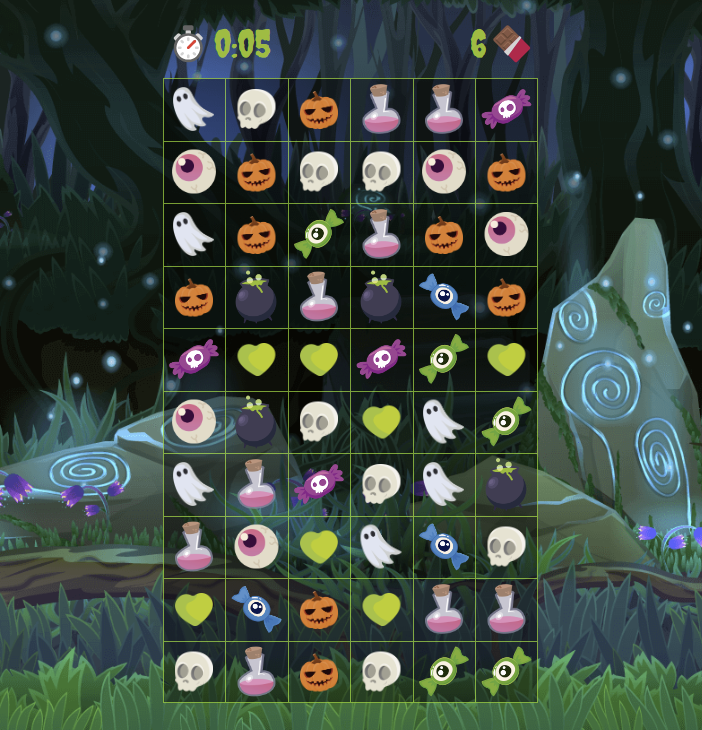
\includegraphics[width=\textwidth]{finished-game.png}

\end{document}